\documentclass{article}
\usepackage[utf8]{inputenc} %obsługa polskich znaków
\usepackage[T1]{fontenc} %obsługa polskich znaków
\usepackage[polish]{babel} %obsługa polskich znakow oraz elementy dokumentu są w języku polskim
\usepackage{indentfirst} %wcięcia akapitów
\usepackage[margin=3cm,nohead]{geometry} %ustawienia strony
\usepackage{listings} %do kodu
\usepackage{booktabs}%do tabel
\usepackage{amsmath}%do wzorow

\usepackage{natbib}
\usepackage{graphicx} %grafika
\usepackage{enumerate}

\title{Laboratorium 10}
\author{Agata Kaczmarek}
\date{January 2021}

\begin{document}
\maketitle 
\newpage
\tableofcontents
\newpage


\section{Rozdział 1 - Zadanie 3}
Jakiś \textbf{pogrubiony} tekst w rozdziale pierwszym.
\subsection{Podrozdział 1}
Inny \texttt{stylizowany kodem} tekst w podrozdziale pierwszym.
\subsection{Podrozdział 2}
Inny \emph{wyróżniony tekst} w podrozdziale drugim rozdziału pierwszego.
\subsubsection{Podpodrozdział 1}
Inny \textit{inaczej wyróżniony}tekst  w podpodrozdziale pierwszym.
\section{Rozdział 2}
Jakiś \textsc{drukowanymi literami} tekst w rozdziale drugim.

\subsection{Podrozdział 1 - Zadanie 4}
Jakiś inny \textnormal{normalny} tekst w podpodrozdziale drugim. \\
Lista egzaminów: 
\begin{enumerate}[a)]
    \item POD
    \item BD
    \item GK
\end{enumerate}
Lista egzaminów: 
\begin{itemize}
    \item C++
    \item Python
    \item Java
    \item C\#
\end{itemize}
\subsection{Podrozdział 2 - Zadanie 5}
Cytując jego słowa ,,Wczoraj oddawaliśmy projekt z IO\footnote{Inżynieria Oprogramowania.}'' .

Obraz:
\begin{figure}[hbt!]
\centering
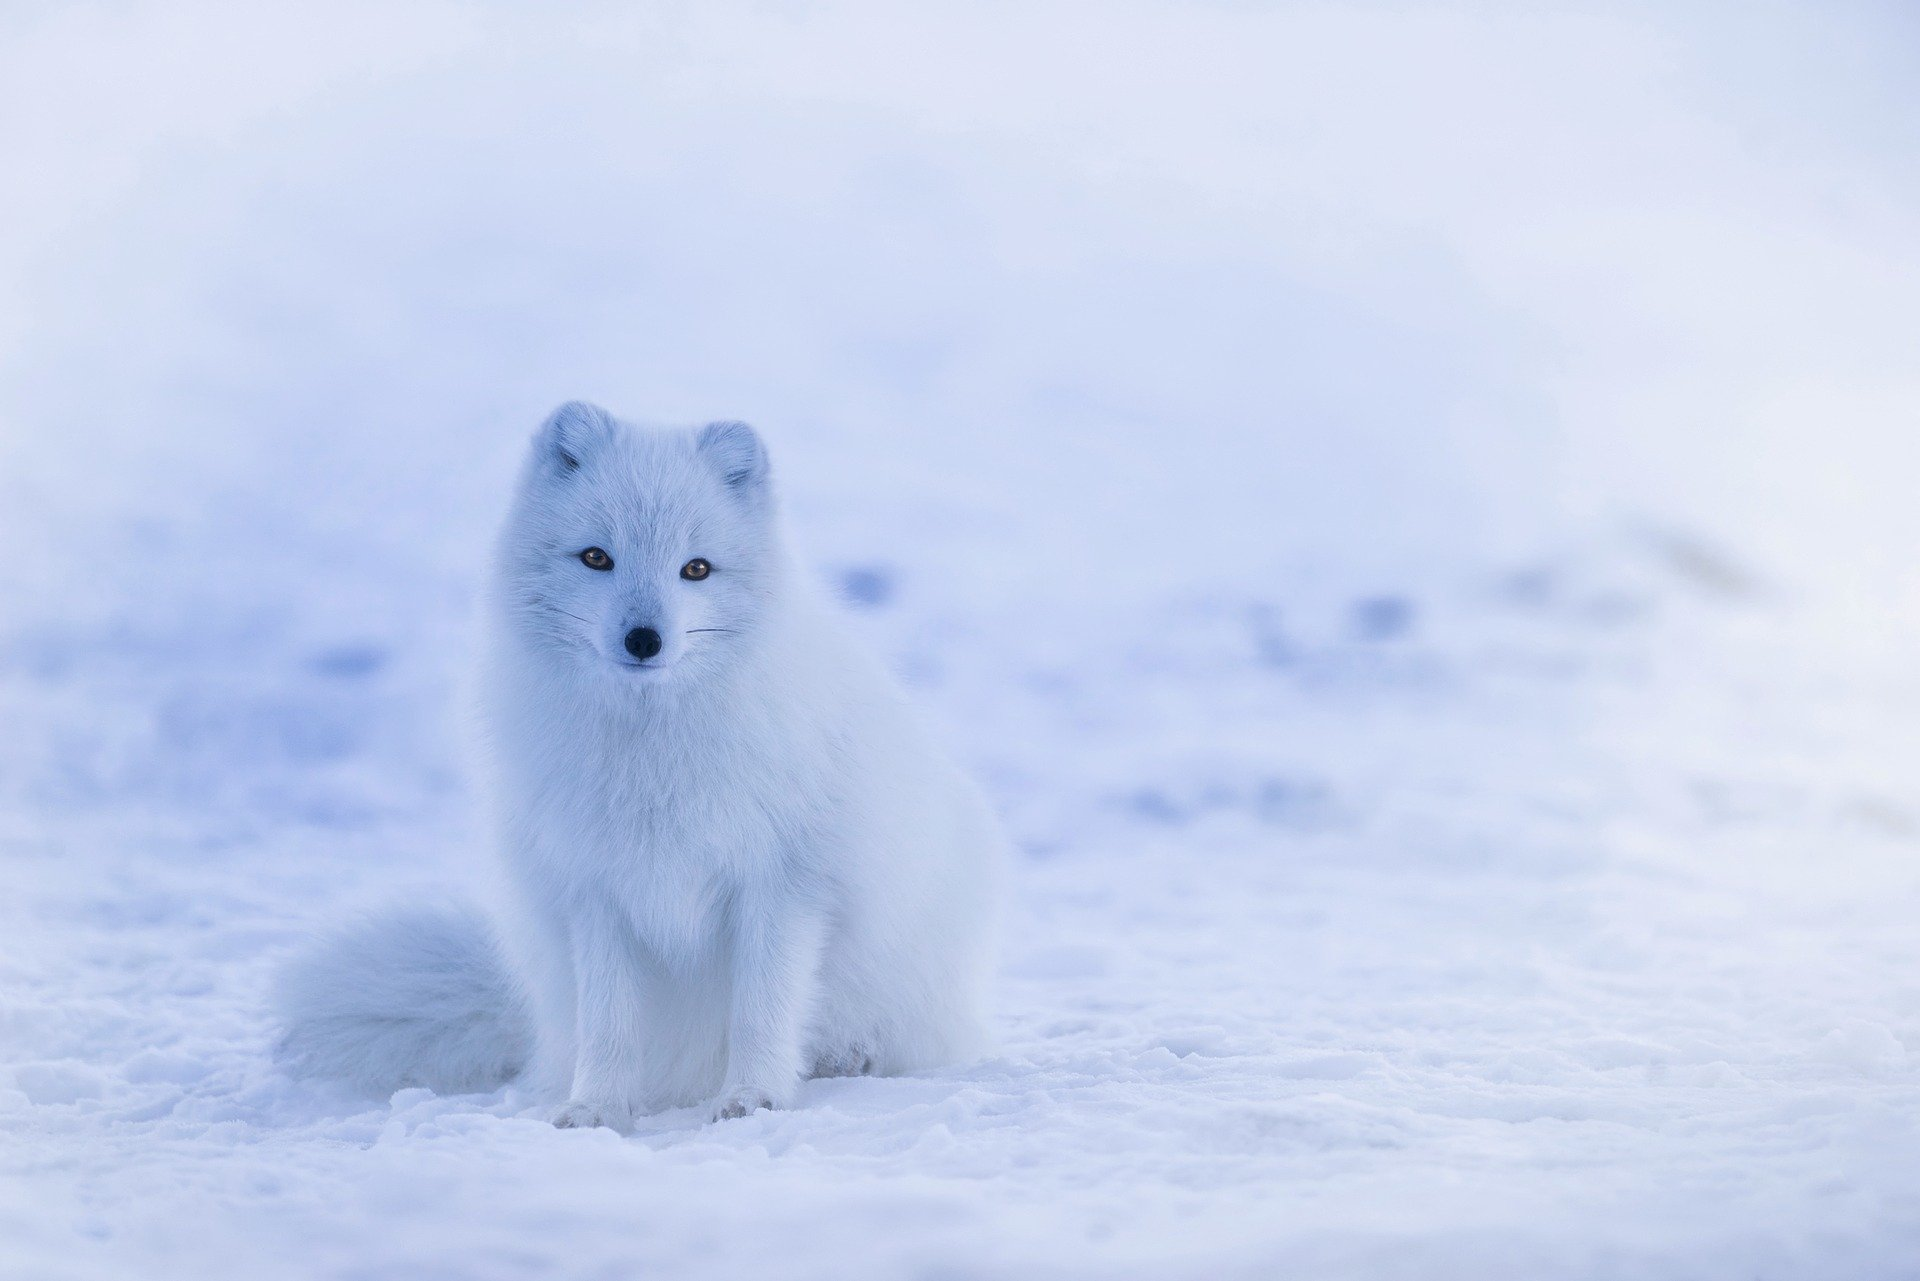
\includegraphics[scale=0.15]{lis}
\caption{Zadanie 6a}
\label{Lis}
\end{figure}

Tabela:
\begin{table}[h!]
\caption{Zadanie 6b}
\label{Tabela województw}
\begin{center}
 \begin{tabular}{|c | c | c|}
 \hline
 Województwo & Powierzchnia & Populacja \\ [1ex] 
 \hline
 dolnośląskie & 19 947 & 2 898 525 \\ 
 \hline
 kujawsko - pomorskie & 17 972 & 2 069 273 \\
 \hline
 lubelskie & 25 122 & 2 103 342 \\
 \hline
 lubuskie & 13 988 & 1 010 177 \\
 \hline
\end{tabular}
\end{center}
\end{table}
\subsection{Podrozdział 3 - Zadanie 6 cd.}
Odwołanie do obrazka: \ref{Lis}
Odwołanie do tablicy: \ref{Tabela województw}

\subsection{Podrozdział 4 - Zadanie 7}
\begin{enumerate}[a)]
    \item $${n\choose k}=\frac{n!}{k!(n-k)!}$$
    \item $$a^{2}+b^{2}=c^{2}$$
    \item $$\frac{\frac{1}{2}+\frac{1}{4}}{\frac{1}{8}}\neq{1}$$
    \item $$\sum_{i=2}^{n}i^{2}=\frac{n(n+1)(n+2)}{6}$$
    \item $$C^{-3}_{2}+O^{0}_{2}\xrightarrow{}C^{+4}+O^{-2}_{2}+H^{+1}_{2}+O^{-2}$$
    \item $$
    \mathbf{A_{m,n}} =
    \left( \begin{array}{cccc}
    a_{1,1} & a_{1,2} & \ldots & a_{1,n} \\
    a_{2,1} & a_{2,2} & \ldots & a_{2,n}\\
    \vdots & \vdots & \ddots & \ldots\\
    a_{m,1} & a_{m,2} & \ldots & a_{m,n} \\
    \end{array} \right)
    $$
\end{enumerate}

\subsection{Podrozdział 5 - Zadanie 8}
\begin{itemize}
    \item ,,Pierwszy cytat'' \citep{ksiazka1} 
    \item ,,Drugi cytat'' \citep{ksiazka2}
    \item ,,Trzeci cytat'' \citep{ksiazka3}
    \end{itemize}



\bibliographystyle{plain}
\bibliography{references}

\end{document}
